

\begin{figure}
    \centering
    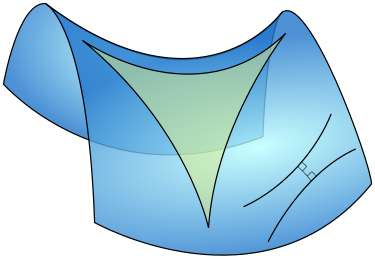
\includegraphics[width=0.4\textwidth]{figs/Hyperbolic_triangle.png}    
    \caption{Section of a hyperbolic space.}
    \label{fig:hyperbolicSpace}
\end{figure}


% \begin{tikzpicture}

% \begin{axis}[view={40}{30}, axis lines=none]
%     \addplot3[
%         surf,
%         colormap/cool,
%         shader=flat,
%         opacity=.6,
%         domain=-10:10,
%         domain y=-10:10,
%         samples=40,
%         clip=false
%         ] {x^2 - y^2};
    
%         \addplot3[
%     color=red, thick, samples=50, domain=-5:5, 
%     samples y=0, smooth
% ] {}


% \addplot3[
%     color=red, thick, samples=10, domain=-5:5, 
%     samples y=0, smooth
% ]
% ({x},   
%  {0},  
%  {x^2}   
% );

% % \addplot3[
% %     color=red, thick, samples=10, domain=-5:5, 
% %     samples y=0, smooth
% % ]
% % ({x},   
% %  {2*x-1},  
% %  {-3*x^2+4*x-1}   
% % );
    
        
    
%     \end{axis}
% \end{tikzpicture}